\documentclass[11pt,oneside]{book}              % Book class in 11 points
\usepackage{amsmath}
\usepackage{amsfonts}
\usepackage{verbatim, graphicx}
\parindent0pt  \parskip10pt             % make block paragraphs
\raggedright                            % do not right justify

\newcommand{\specell}[2][c]{%
  \begin{tabular}[#1]{@{}c@{}}#2\end{tabular}}
\newcommand\Tstrut{\rule{0pt}{2.6ex}}         % = `top' strut
\newcommand\Bstrut{\rule[-0.9ex]{0pt}{0pt}}   % = `bottom' strut

\title{\bf Mathematical Function Theory}    % Supply information
\author{Juan Vallejo}              %   for the title page.
\date{\today}                           %   Use current date. 

% Note that book class by default is formatted to be printed back-to-back.
\begin{document}                        % End of preamble, start of text.
\frontmatter                            % only in book class (roman page #s)
\maketitle                              % Print title page.
\tableofcontents                        % Print table of contents
\mainmatter                             % only in book class (arabic page #s)
\chapter{Mathematical Function Theory}                % Print a "chapter" heading
This book chapter contains a brief introduction to the history of functions and their application in the workplace, as well as functions commonly encountered in single variable calculus.

The concept of functions emerged in the 17th century in connection with the development of calculus. Functions eventually went from being defined as an analytic expression to a single-valued mapping from one set to another. The term \textit{function} was introduced by \textbf{Gotffried Leibniz} in 1673 in order to describe any quantity related to a curve; such as a curve's slope at a specific point. Leibniz later went on to re-define functions as \textit{any expression made up of a variable and some constants}. These functions are classified today as \textit{differentiable functions}. Functions eventually received their familiar notation $f(x)$ after Leonhard Euler introduced the expression in 1744 \cite{euler1}.

\section{Introduction}                  % Print a "section" heading
In mathematics, a function is a relation between a set of inputs and a set of permissible outputs with the property that each input is related to exactly one output \cite{wolfram1}.

Function theory is an integral part of mathematics and the computational world. It allows us to use the same set of rules more than once in an expression, with different parameter values, and recognize similarities in a set of observations. This theory is implemented by programming languages such as Haskel, as part of a new programming language paradigm, in order to perform calculations without mutating memory \cite{mathexchange2}.

To illustrate an example of the usefulness of functions in real-world problem solving, consider a scenario where $x$ represents the number of days since a local factory became operational and $y$ represents the number of accidents that have occurred at that same factory. Suppose we want to figure out the average number of accidents per day in the current month. We don't know the \textit{actual values} yet (as we are still in the current month), but we can aim to write down a formula that tells us what to do \textit{once} we have the numbers. Then we need to subtract the number of accidents on the first day of the current month from the number of accidents on the first day of the following month and divide it by the number of days that came in between. However, those two numbers of accidents are both values of $y$, so if all we have is the variables themselves, we end up with $\frac{y - y}{30}$ (assuming that the current month has $30$ days) which is nonsense. However, if we define a \textit{function} $f$ as \textit{the $y$ corresponding to day $x$}, we can now write the average as:
\begin{equation*}
	\frac{f(60) - f(31)}{30}
\end{equation*}
which then tells us unambiguously what to do. A significant advantage of the example above is that we can now use our concept of a function to recognize similarities. If we have four variables $x, y, z, w$, and it turns out that there is a function $f$ such that $y = f(x)$ and $z = f(w)$ for all corresponding values of the four variables, this tells us mainly that the \textit{relation} between $x$ and $y$ is the same as the relation between $w$ and $z$.

\section{Components and Relations}
Functions can be seen as relations that uniquely associate members of one set with members of another set. More formally, a function from $A$ to $B$ is an object $f$ such that every $\alpha \in A$ is uniquely associated with an object $f(a) \in B$. A function, by this observation, can be seen as a many-to-one relation \cite{wolfram2}.

\subsection{Domain and Range}
The set $A$ of values at which a function is defined is called its \textit{domain}, while the set $f(A) \subset B$ of values that the function can produce is called its range \cite{wolfram2}. It is usually a union of intervals, and is denoted by $D(f), D_f$, or $dom(f)$:
\begin{equation*}
	D(f) = \lbrace \in \mathbb{R}; f(x) \rbrace
\end{equation*}

The \textit{range} of a function is the set of all values that can be obtained by substituting arguments from the domain.

\subsection{Mapping}
In mathematics, the term \textbf{map} is often used to refer to functions. It can be used to denote functions with regular assumptions, such as in the case of continuous functions. In \textit{category theory}, ``map" is often used as a synonym for \textit{morphism}. In other words, it is used to specify something more general than a function \cite{cattheory}. In \textit{formal logic}, a map is used at times to declare a \textit{functional predicate}, whereas a function is a model of such a predicate in \textit{set theory}.

\subsection{Real Functions}
A function is defined as ``real" when $f: A \subset \mathbb{R} \to \mathbb{R}$. The fact that domain elements are mapped to unique range elements can be expressed graphically by performing the vertical line test. Real functions are the most important type of \textit{mapping}. They can be thought of as any mapping from some subset of the set of real numbers to the set of real numbers \cite{mathfeld}.

\subsubsection{Basic Notions}
A real function can be thought of as a prescription which assigns values to arguments. For example, the notation $y = f(x)$ means that to the value $x$ of the argument, the function $f$ assigns the value $y$. A second notation $f: x \to y$ is also used, which implies that the function $f$ sends value $x$ to $y$. The most usual way of specifying assignments is that the function value $y$ can be obtained by substituting $x$ to a specific formula that identifies the given function. For example,
\begin{equation*}
f(x) = 2x + 3
\end{equation*}
would send the argument $x = -1$ to $f(-1) = 2 \cdot (-1) + 3 = 1$

\subsubsection{Substitution}
The formula form of a function can be considered simply as a recipe for what to do with a given input. The input, given as the function's argument, is \textit{substituted} into the function declaration in order to define the process of retrieving an output. It is not uncommon, especially in calculus, to use the formula form of a function with a \textit{mathematical expression} as its argument instead of a number or single variable. Consider the following example:
\begin{equation*}
	f(x) = x^2 - 2x
\end{equation*}
This expression basically means that the function value is gotten by taking the square of the argument and subtracting twice the argument from it. It does not matter what symbol we use for the argument; rather it is how the function works that is of importance. The following items are valid examples of function substitutions:
\begin{itemize}
	\item $f(4) = 4^2 − 2 \cdot 4 $
	\item $f(t) = t^2 − 2t$
	\item $f(x + h) = (x+ h)^2 − 2 (x + h)$
	\item $f(a x) = (a x)^2 − 2 (a x)$
\end{itemize}

Just as we can substitute an expression into a function, so we can substitute function into another function, for example:
\begin{align}
	f(x) &= x^2 - 2x \\
	g(x) &= x + 3 \\
	f(g(x)) &= (g(x))^2 - 2g(x) \\
	f(g(x)) &= (x + 3)^2 - 2(x + 3)
\end{align}
This concept will be covered more in-depth later on in this chapter.

There is an alternative way to express the idea that we substitute some concrete number into a function:
\begin{equation*}
f(a) = f \mid_a = f\mid_{x=a}
\end{equation*}
This notation is specially used when a function needs adjustment, but is not yet ready for substitution. For example:
\begin{equation*}
\left.\frac{x^2 - 1}{x-1}\right\rvert_{x=3} = \left.\frac{(x-1)(x+1)}{x-1}\right\rvert_{x=3} = 4.
\end{equation*}

\subsubsection{Visualization}
Graphs are a common way of visualizing functions in mathematics. They are used to mark in the two-dimensional plane $(x,y)$ all couples $x, f(x)$ \cite{mathfeld}. Below is an example of the function $y=ax^2+bx+c$ when $a = 1, b = 0, \text{and} c = 1$:
\begin{center}\includegraphics[scale=0.5]{Function_Graph_Draft_Sine.png}\end{center}

\section{Types of Functions}
Functions are the primary objects of study in calculus, consisting of various types, from \textit{linear} to \textit{polynomial}, \textit{trigonometric}, and \textit{logarithmic}. \cite{oregonstate}

\subsection{Linear Functions}
Linear functions allow us to approximate more complicated functions in differential calculus. There are three standard forms of linear functions:
\begin{align*}
f(x) &= mx + b &\,\text{(Slope-intercept form)} \\
y - y_o &= m(x - x_0) &\, \text{(The ``point-slope" form)} \\
Ax + By &= C &\, \text{(The ``general" form)}
\end{align*}

\subsubsection{Calculations}
Linear functions are frequently used to solve for the following calculations:
\begin{itemize}
	\item {\bf Intercepts} - Finding the slope, x-intercept, and y-intercept of the line given its equation.
	\item {\bf Intersections } - Finding the intersection of two lines from their equations.
	\item {\bf Equations } - Finding the equation of the line through a series of points given one of the following three pairs of data:
	\begin{itemize}
		\item the slope of the line and the y-intercept
		\item the slope of the line and a point $(x_0,y_0)$ on the line
		\item the coordinates of two points on the line
	\end{itemize}
\end{itemize}

Consider an example where we are given the equation for a line. The x-intercept is determined by setting $y=0$, the y-intercept is determined by setting $x = 0$, and the slope is determined by putting the equation into the form $y = mx + b$. The slope is then $m$. If the equation of the line is:
\begin{equation*}
	y - 2 = 3(x + 4)
\end{equation*}

the x-intercept is found by setting $y = 0$ and solving for $x$:
\begin{align}
	-2 &= 3(x + 4)\\
	-2 &= 3x + 12\\
	-14 &= 3x\\
	x &= \frac{-14}{3}
\end{align}

The y-intercept is found by setting x=0 and solving for y:
\begin{align}
	y - 2 &= 3(4)\\
	y - 2 &= 12\\
	y &= 14
\end{align}

The slope is found by re-writing the equation:
\begin{align}
	y - 2 = 3x+12
\end{align}

In the \textit{slope-intercept} form ($y = mx + b$), we can easily see that the slope of the graph is $3$.

\subsubsection{Graphs}
If $f(x)$ is linear, the graph of $y=f(x)$ is a straight line. The parameter $m$ in the first two formulas represents the slope of this line. In the general form, the slope is $-A/B$ if $B \neq 0$, and indefinite if $B=0$ \cite{oregonstatelinear}.
An example of the graph of $f(x)$ when $x = 1$ is illustrated below:
\begin{center}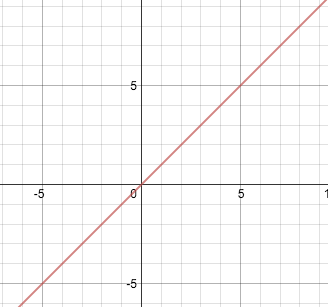
\includegraphics[scale=0.5]{Function_Graph_Draft.png}\end{center}

\subsection{Polynomial Functions}
Polynomial functions can be represented as a function $f(x)$ by a formula:
\begin{equation*}
	f(x) = a_nx^n + a_{n-1}x{n-1} + \cdots a_1x + a_0
\end{equation*}
where $a_0, a_1$, \dots , $a_n$ are real numbers. These are called the coefficients. It is assumed that $a_n \neq 0$. The number $n$ is called the degree of the polynomial function. It is defined as the largest exponent of $x$ which appears in the polynomial. It is also the subscript of the leading term. If a polynomial consists of only a single term, it is called a \textbf{monomial}. If the polynomial's degree is $0$, then the polynomial is defined as a constant. Otherwise, if its degree is $1$, then it is defined as a linear function. Polynomials with degrees greater than one are defined as \textit{quadratic} if the degree is $2$, \textit{cubic} if the degree is $3$, \textit{quartic} if the degree is greater than $4$, and so on.

The behavior of a polynomial function, regardless of the size of its degree, is exactly the same as the behavior of its monomial over a large enough scale.

\subsubsection{Graphs}
The general shape of the graph of a monomial
\begin{equation*}
	f(x) = a_nx^n
\end{equation*}
depends only on
\begin{itemize}
	\item The parity of $n$ (whether $n$ is even or odd)
	\item The sign of $a_n$
\end{itemize}

For the example above, as $n$ gets larger, all of the equation's graphs become increasingly flat on the interval $\vert x\vert < 1$. All polynomial functions grow without bound in a positive or negative direction for large $x$ and large negative $x$.

\begin{center}
\begin{tabular}{ c c c }
  & Graph of even $n$ & Graph of odd $n$ \\ \hline 
 $a_n > 0$ & \specell{Always positive. \\ Resembles parabola opening up.} & \specell{Negative for $x < 0$\\Positive for $x > 0$ \\Resembles graph of $x^3$.} \\ 
 $a_n < 0$ & \specell{Always negative. \\ Resembles parabola opening down.} & \specell{Positive for $x < 0$\\Negative for $x > 0$ \\Resembles graph of $-x^3$.}
\end{tabular}
\end{center}

\subsection{Power \& Exponential Functions}
\subsubsection{Power Functions}

Power functions are of the form:
\begin{equation*}
  f(x) = kx^p
\end{equation*}
where $p$ is any real number and $k$ is non-zero.

If p is a non-zero integer, then the domain of the power function $f(x) = kx^p$ consists of all real numbers. For rational exponents $p, x^p$ is always defined for positive $x$. However an even root of a negative number can not be extracted, thus an expression such as $x^{\frac{1}{4}}$ is not defined for any negative real numbers.

Any rational number $p$ can be written in the form $p = \frac{r}{s}$ where all common factors of $r$ and $s$ have been canceled. At this point, an expression $kx^p$ has a domain of \textit{all real numbers} if $s$ is odd, or \textit{All non-negative real numbers} if $s$ is even.

\subsubsection{Exponential Functions}
Exponential functions are functions of the form $f(x) = b^x$ for a fixed base $b$ which can be any \textit{positive real number}. They are characterized by their rate of growth, which is proportional to their value. A distinguished type of exponential function is of the form $f(x) = e^x$. Its rate of growth at $x$ is exactly equal to the value $e^x$ of the function at $x$. The number $e$ is named after Leonid Euler, whom we introduce at the beginning of this chapter as the father of the function's mathematical notation $f(x)$ \cite{oregonstateexp}.

Exponential functions differ from \textit{power functions} in that power functions have constant exponents; in exponential functions, an exponent $x$ will vary.
\begin{center}\includegraphics[scale=0.5]{../Function_ExpoGraph_slOther.png} \end{center}

\subsubsection{Rules of Exponentiation}
The main rules of exponentiation are as follows:
\begin{itemize}
	\item $x^{(p + q)} = (x^p)(x^q)$
	\item $x^{pq} = (x^p)^q$
	\item $x^{-p} = \frac{1}{x^p}$
	\item $x^{\frac{1}{p}}$ is the $p$-th root of $x$
	\item $x^0 = 1$ for any $x\neq 0$. $0^0$ is undefined
	\item $(x^y)^p = (x^p)(y^p)$
\end{itemize}

Root functions such that $f(x) = \sqrt{x}$ are really just special cases of power functions. An example of this is$\sqrt{x} = x^{\frac{1}{2}}$.

Additional rules commonly used in manipulation exponential functions are as follows:
\begin{itemize}
	\item $b^{x + y} = (b^x)(b^y)$
	\item $b^{xy} = (b^x)^Y$
	\item $b^0 = 1$
	\item $b^{-x} = \frac{1}{b^x}$
\end{itemize}

\subsection{Rational Functions}
Rational functions can be represented as the quotient of polynomials, similarly to  rational numbers being represented as quotients of whole numbers. All polynomials are rational functions. They can be thought of as rational expressions with $1$ as their denominator.

The typical form of a rational function is $\frac{p(x)}{a(x)}$ where $p$ and $q$ are polynomials. $p(x)$ is the numerator and $q(x)$ is the denominator.

Consider the following example:
\begin{equation*}
  g(x) = \frac{x^2 - 4}{x^2 - 5x + 6}
\end{equation*}
In the example illustrated above,  $x^2 - 4$ is the numerator and $x^2 - 5x + 6$ is the denominator.

\subsubsection{Domain and Range}
The domain of a rational function $\frac{p(X)}{q(x)}$ consists of all points where $q(x)$ is non-zero. Domains such as this one ultimately depend on the way in which $p(x) and q(x)$ are chosen. For example, the function $g(x)$ stated above can be written as:
\begin{equation*}
	g(x) = \frac{(x-2)(x+2)}{(x-3)(x-2)}
\end{equation*}
This example eventually simplifies to $\frac{(x+2)}{(x-3)}$. Despite this, $x=2$ is not considered the domain of the function $g(x)$. But it is the domain of its simplified form; $\frac{(x+2)}{(x-3)}$.

\section{Other Functions}
\subsection{Logarithmic Functions}
Logarithmic functions are defined as any function of the form $\log_bx$ being the inverse function of the exponential function $b^x$. There are three main bases for logarithms:
\begin{itemize}
	\item \textbf{Natural logarithms} written as $\ln x$, expressed as the logarithm to the base $e$. Thus $e^x$ and $\ln(x)$ are inverse functions
	\item \textbf{Common logarithms} written as $\log x$, expressed as the logarithm to the base $10$. Thus $10^{\log x} = x$
	\item \textbf{Binary logarithms} used in communications and computer science with a base of $2$. Expressed as $\log(x)$ or $\log_2x$ where $x$ is an integer measuring the number of bits it takes to write $x$.
\end{itemize}
\begin{center}\includegraphics[scale=0.5]{../Function_LogGraph_slOther.png} \end{center}

\subsection{Trigonometric Functions}
Trigonometric functions link calculus to geometry. All trigonometric functions are functions of radians. Examples include $sin(x)$ and $cos(x)$:
\begin{center}\includegraphics[scale=0.9]{../Function_TrigCircl_slOther.png} \end{center}

Below are examples of other well-known trigonometric functions:
\begin{itemize}
	\item $\tan(x) = \frac{\sin(x)}{\cos(x)}$
	\item $\cot(x) = \frac{\cos(x)}{\sin(x)}$
	\item $\sec(x) = \frac{1}{\cos(x)}$
	\item $\csc(x) = \frac{1}{\sin(x)}$
\end{itemize}

\begin{center}\includegraphics[scale=0.5]{../Function_SinCos_slOther.png} \end{center}
An illustration of sine and cosine waves is depicted above.

\section{Function Composition}
Composition is the operation of taking the output from one function and using that as the input to a second function. It, together with the algebraic operations on functions, is what allows us to take the basic building blocks of ``pure" function types and build large varieties of functions which is the focus of calculus.

\subsubsection{Definition}
The composition $f \circ g$ of the two functions $f$ and $g$ is the function which feeds an input to $g$ and feeds the output of $g$ to $f$. For example, lets define the following function:
\begin{equation*}
	f(x) = x^2 − 2x
\end{equation*}

If we substitute a second function $g(x)$ into the above function, we get:
\begin{equation*}
	f(g(x)) = (g(x))^2 - 2g(x)
\end{equation*}

If we then define the function $g(x)$ as $g(x) = x + 3$ then:
\begin{equation*}
	f(g(x)) = (x + 3)^2 - 2(x+3)
\end{equation*}

Alternatively, the order of substitution can be switched so that \textit{function $f$ goes into function $g$}:
\begin{align}
	g(f(x)) &= f(x)\\
	g(f(x)) &= (x^2 - 2x) + 3
\end{align}
Note that both results obtained by substituting $f(x)$ and $g(x)$ into each other are completely different. The compositions of functions is important because with this method we can create complex functions out of simple components.

\section{Real-World Applications}
Mathematical function theory is used in the design of various programming languages. The intent of using such concept as a basis in a different approach to the design of programming languages gives way to several advantages and disadvantages not seen with procedural and object-oriented programming. Examples of purely functional programming languages include:
\begin{itemize}
	\item{Haskell}
	\item{Agda}
	\item{Mercury}
\end{itemize}
It is further used in every-day life when computing things such as \textbf{miles per gallon}, or \textbf{weekly salaries}, or \textbf{compound interest}. These are all functions of specific rates such as hourly pay for salaries, or initial investment and interest rate over time for compound interest.

\section{Chapter Conclusion}
Mathematical Function theory is an important part of mathematics and of the world around us. It has a rich history, evolution, and application in mathematics. Function theory is made up of a plethora of sub-sections consisting of different functions, cases, and rules. It is used every day in applications like the stock market, to calculating monthly budgets, to rendering computer graphics.
\begin{center}\includegraphics[scale=0.5]{../Function_CompGraphics_slLast.jpg} \end{center}

\begin{thebibliography}{10}

\bibitem{wolfram1} http://mathworld.wolfram.com/Function.html
\bibitem{wolfram2} http://functions.wolfram.com/ElementaryFunctions/
\bibitem{oregonstate} http://oregonstate.edu/instruct/mth251/cq/FieldGuide/
\bibitem{oregonstatelinear} http://oregonstate.edu/instruct/mth251/cq/FieldGuide/linear/lesson.html
\bibitem{oregonstateexp} http://oregonstate.edu/instruct/mth251/cq/FieldGuide/exponential/lesson.html
\bibitem{mathexchange1} http://math.stackexchange.com/questions/575198/what-purpose-does-the-use-of-functions-serve-in-mathematics
\bibitem{mathexchange2} http://math.stackexchange.com/questions/108133/what-are-functions-used-for
\bibitem{mathfeld} http://math.feld.cvut.cz/mt/txtb/3/txeba3a.htm
\bibitem{cattheory} https://books.google.com/books?id=VOCQUC\_uiWgC\&pg\=PA2\&hl=en\#v=onepage\&q\&f=false
\bibitem{mathonweb} http://mathonweb.com/help\_ebook/html/functions\_6.htm\#expr
\bibitem{euler1} http://mathsforeurope.digibel.be/Euler.html

\end{thebibliography}

\end{document}                          % The required last line
